\subsection{External Interface Requirements}
\subsubsection{User Interfaces}
\begin{figure}[H]
    \centering
    \caption{User Login}
    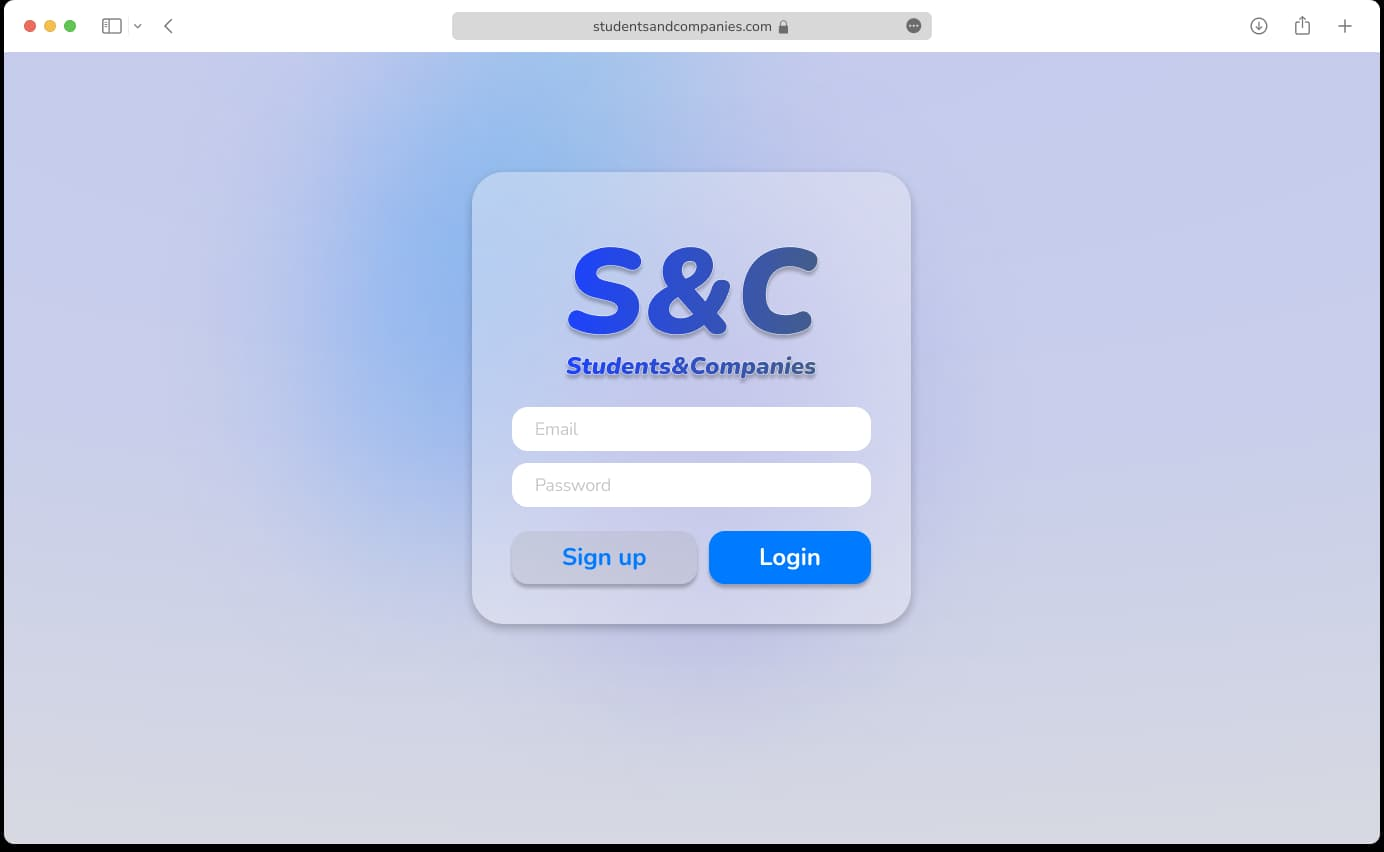
\includegraphics[width=0.8\textwidth]{Images/MockUps/login.jpeg}
    \label{fig:enter-label}
\end{figure}
\newpage
\begin{figure}[H]
    \centering
    \caption{Edit Profile}
    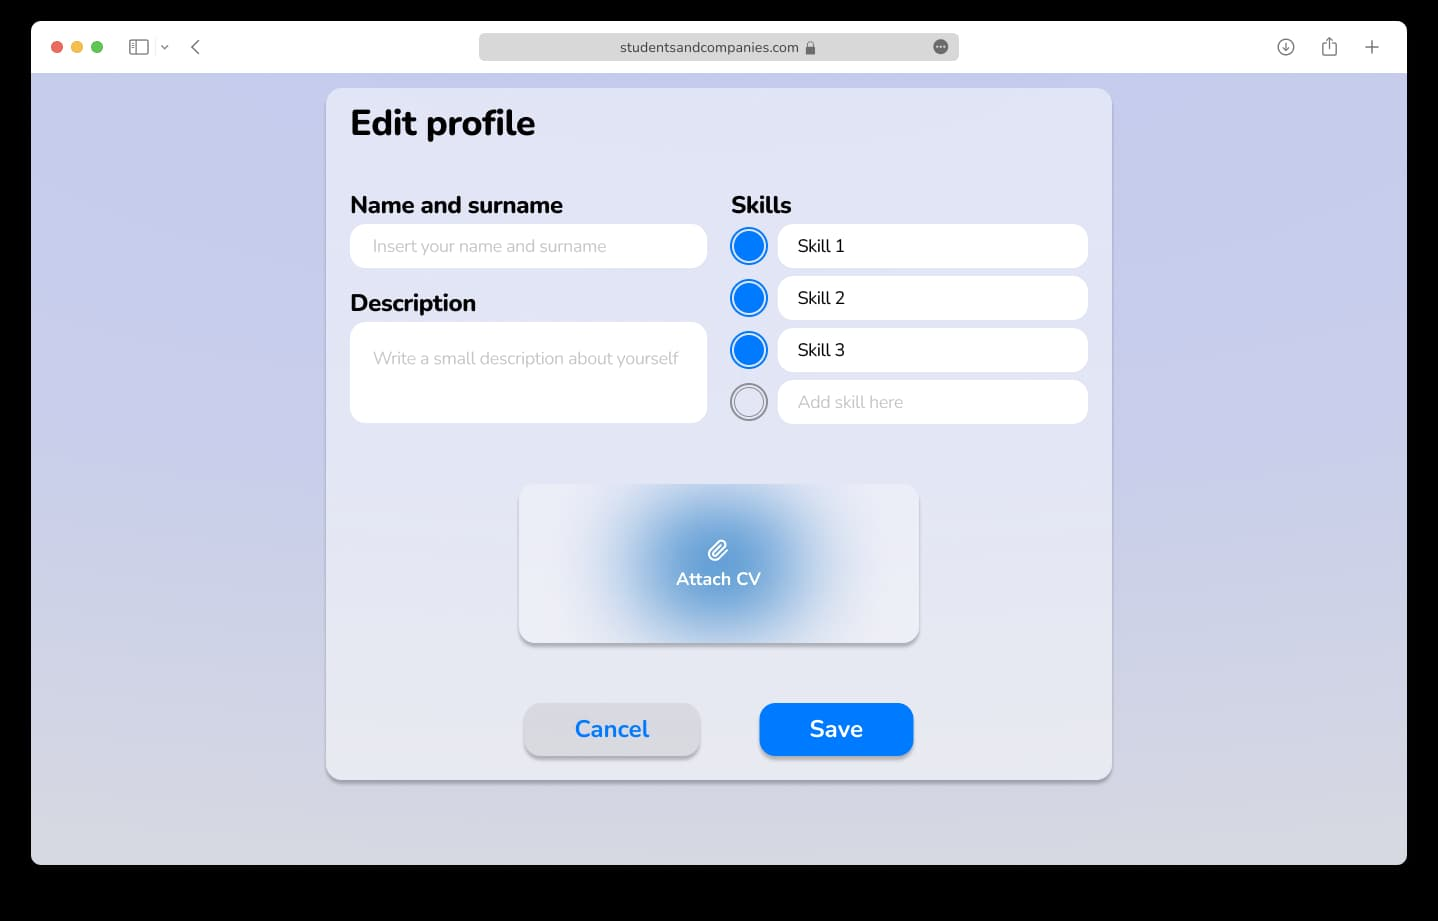
\includegraphics[width=\textwidth]{Images/MockUps/edit_profile.jpeg}
    \label{fig:enter-label}
\end{figure}
\begin{figure}[H]
    \centering
    \caption{Search Internship}
    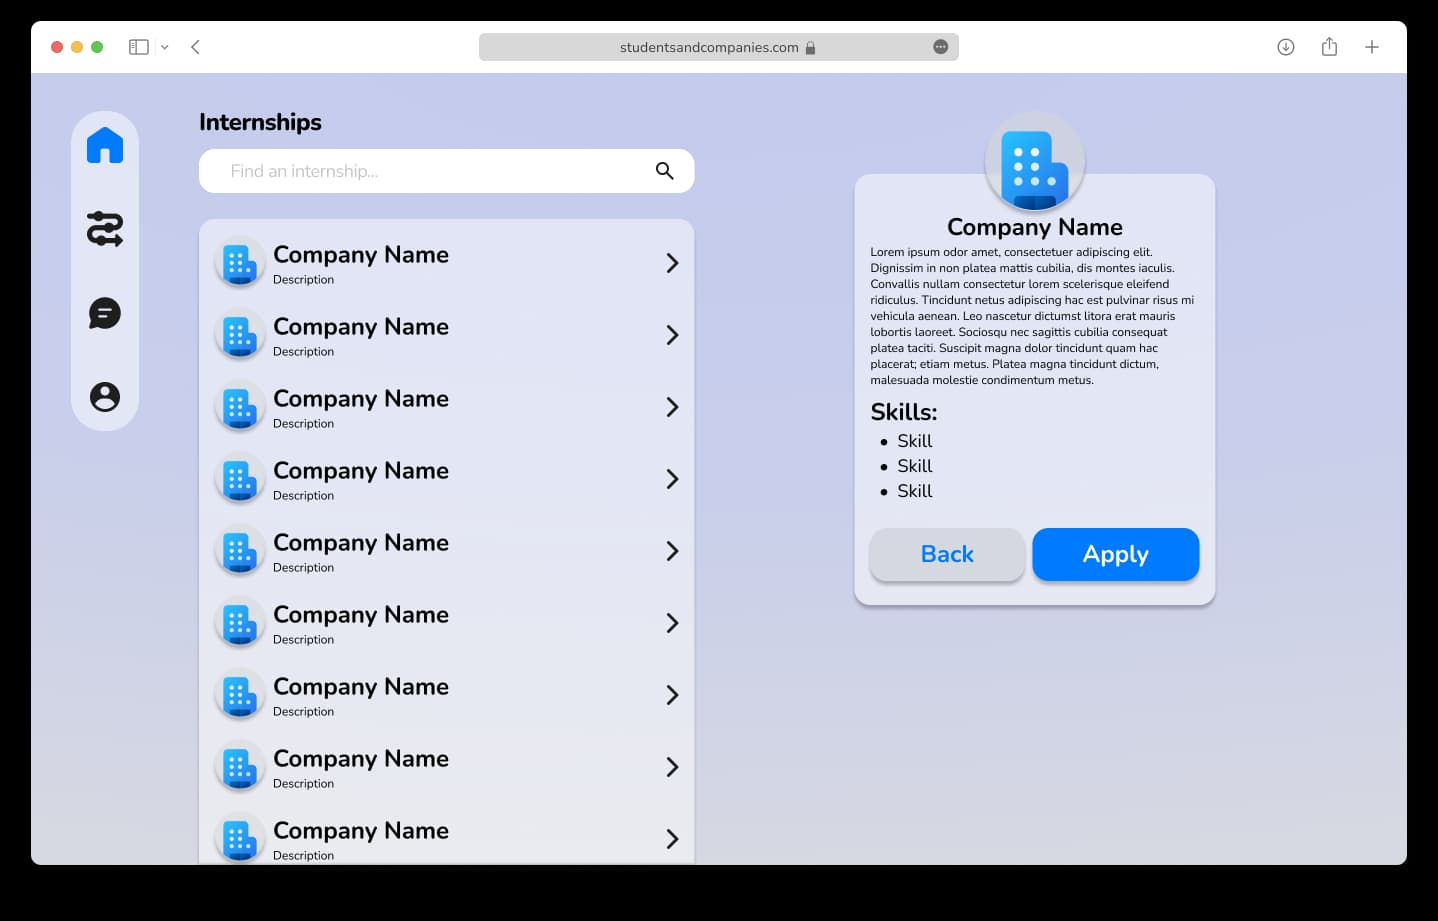
\includegraphics[width=\textwidth]{Images/MockUps/search_internship.jpeg}
    \label{fig:enter-label}
\end{figure}
\begin{figure}[H]
    \centering
    \caption{Create Questionnaire}
    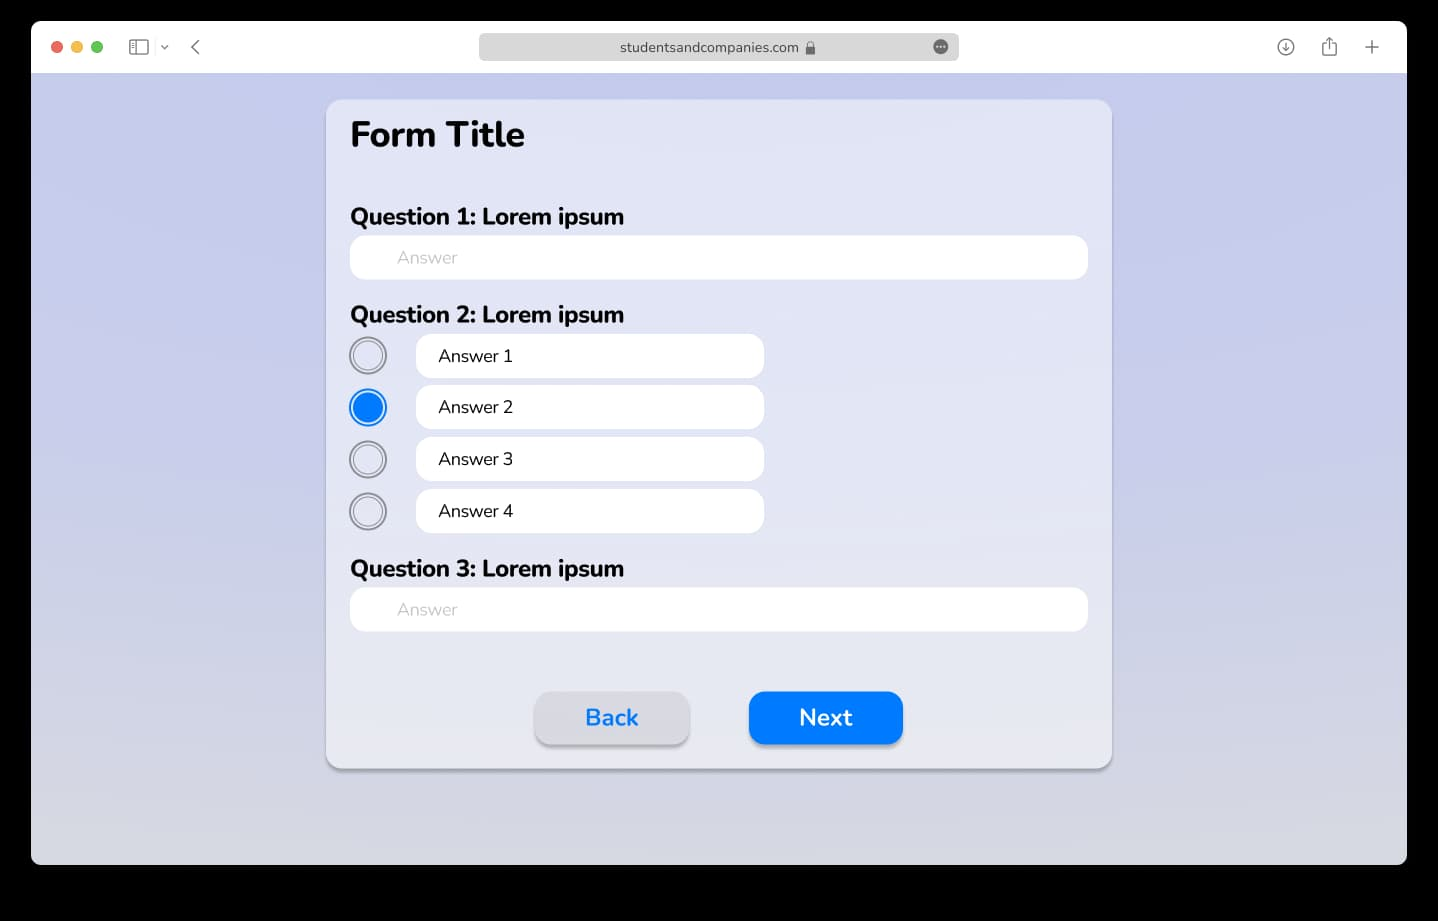
\includegraphics[width=\textwidth]{Images/MockUps/create_questionnaire.jpeg}
    \label{fig:enter-label}
\end{figure}
\begin{figure}[H]
    \centering
    \caption{Discussion}
    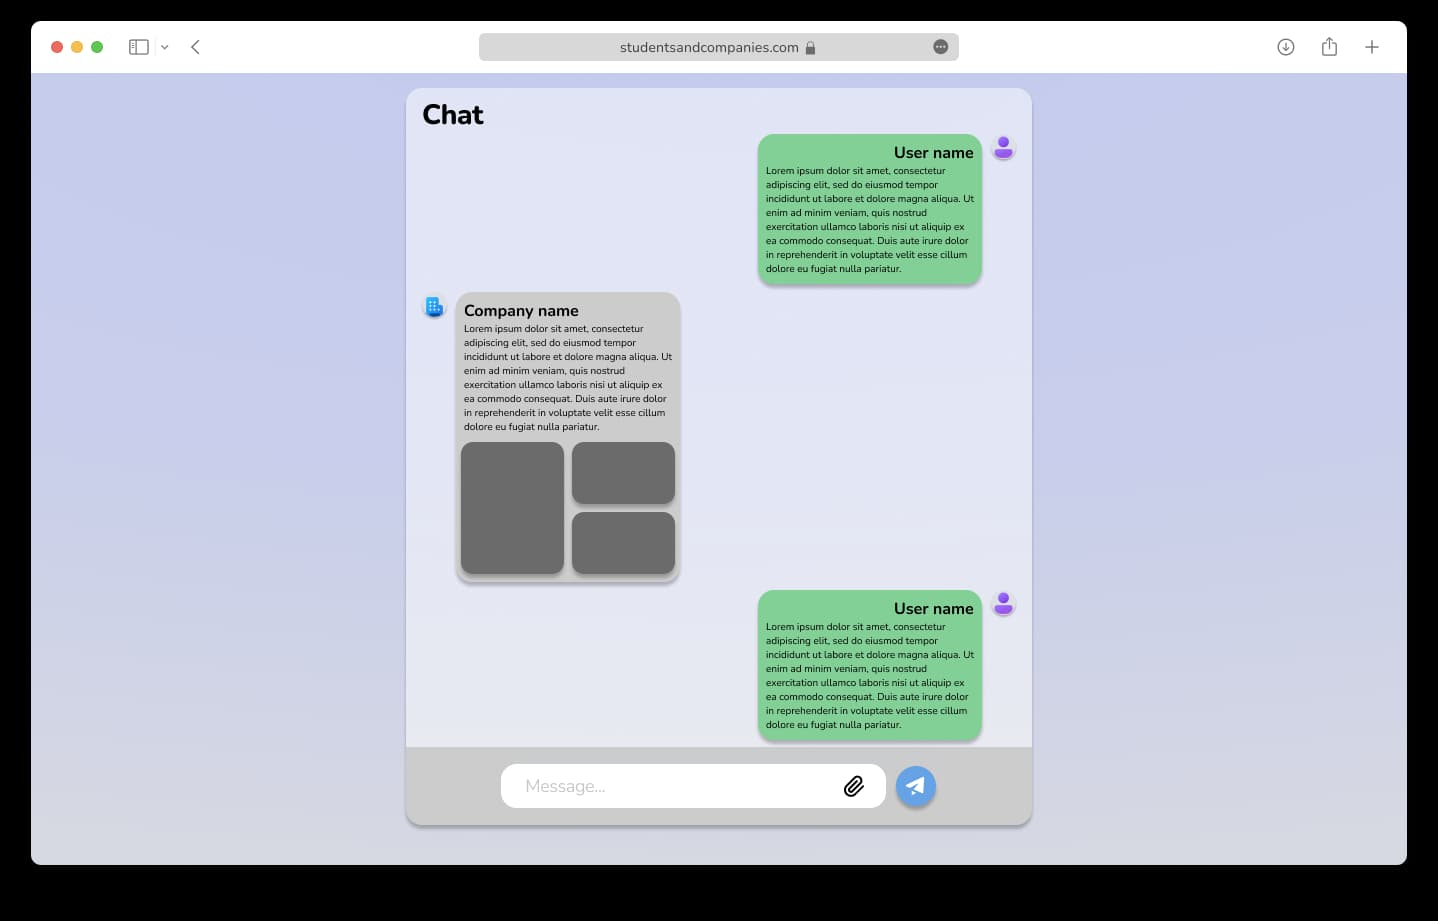
\includegraphics[width=\textwidth]{Images/MockUps/discussion.jpeg}
    \label{fig:enter-label}
\end{figure}
\begin{figure}[H]
    \centering
    \caption{Upload Internship}
    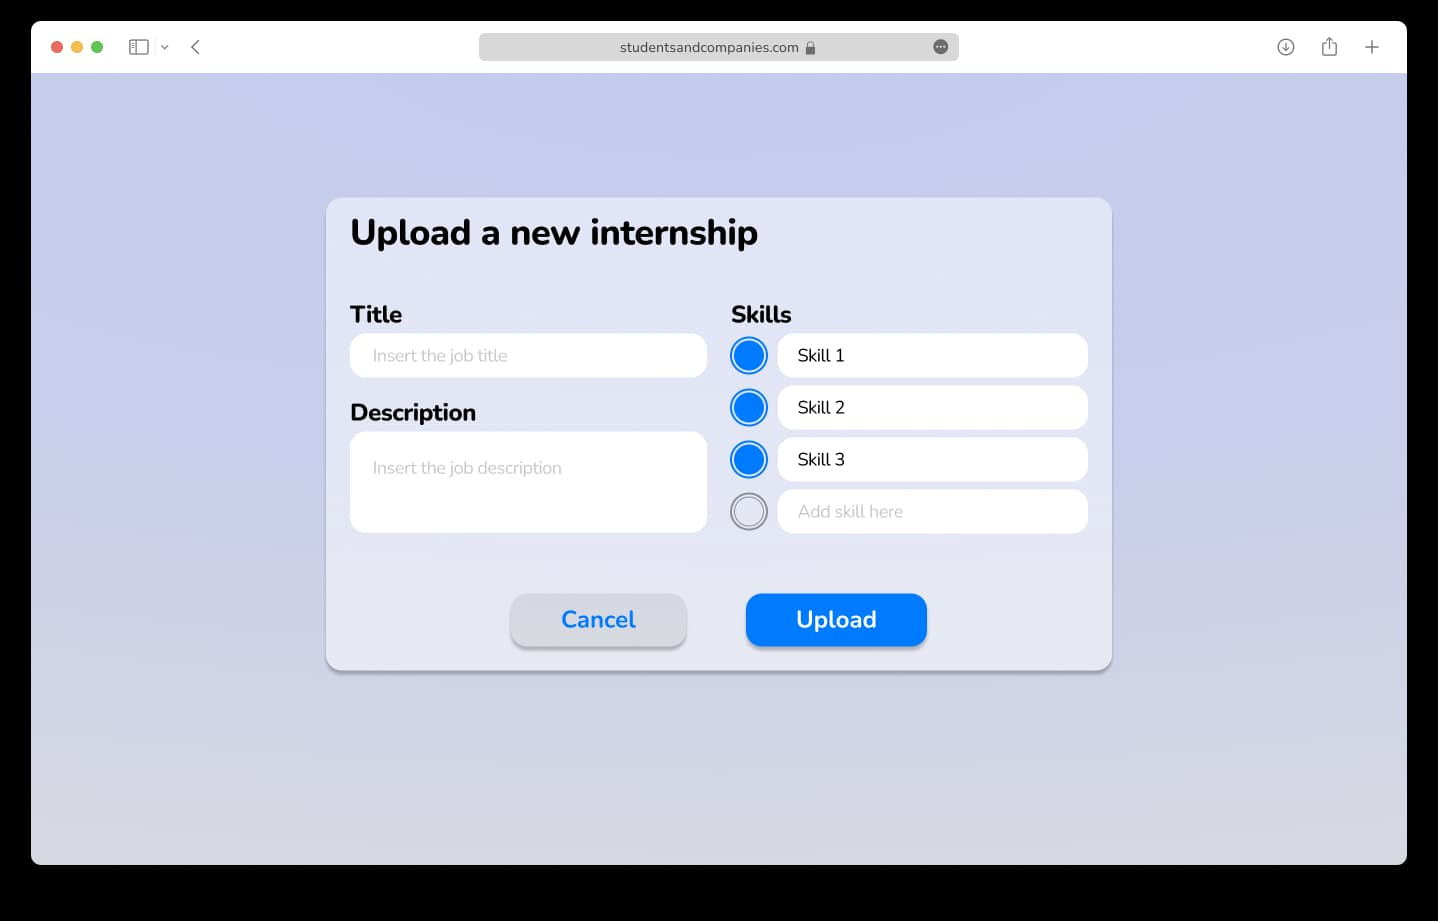
\includegraphics[width=\textwidth]{Images/MockUps/upload_internship.jpeg}
    \label{fig:enter-label}
\end{figure}
\begin{figure}[H]
    \centering
    \caption{Monitor Status}
    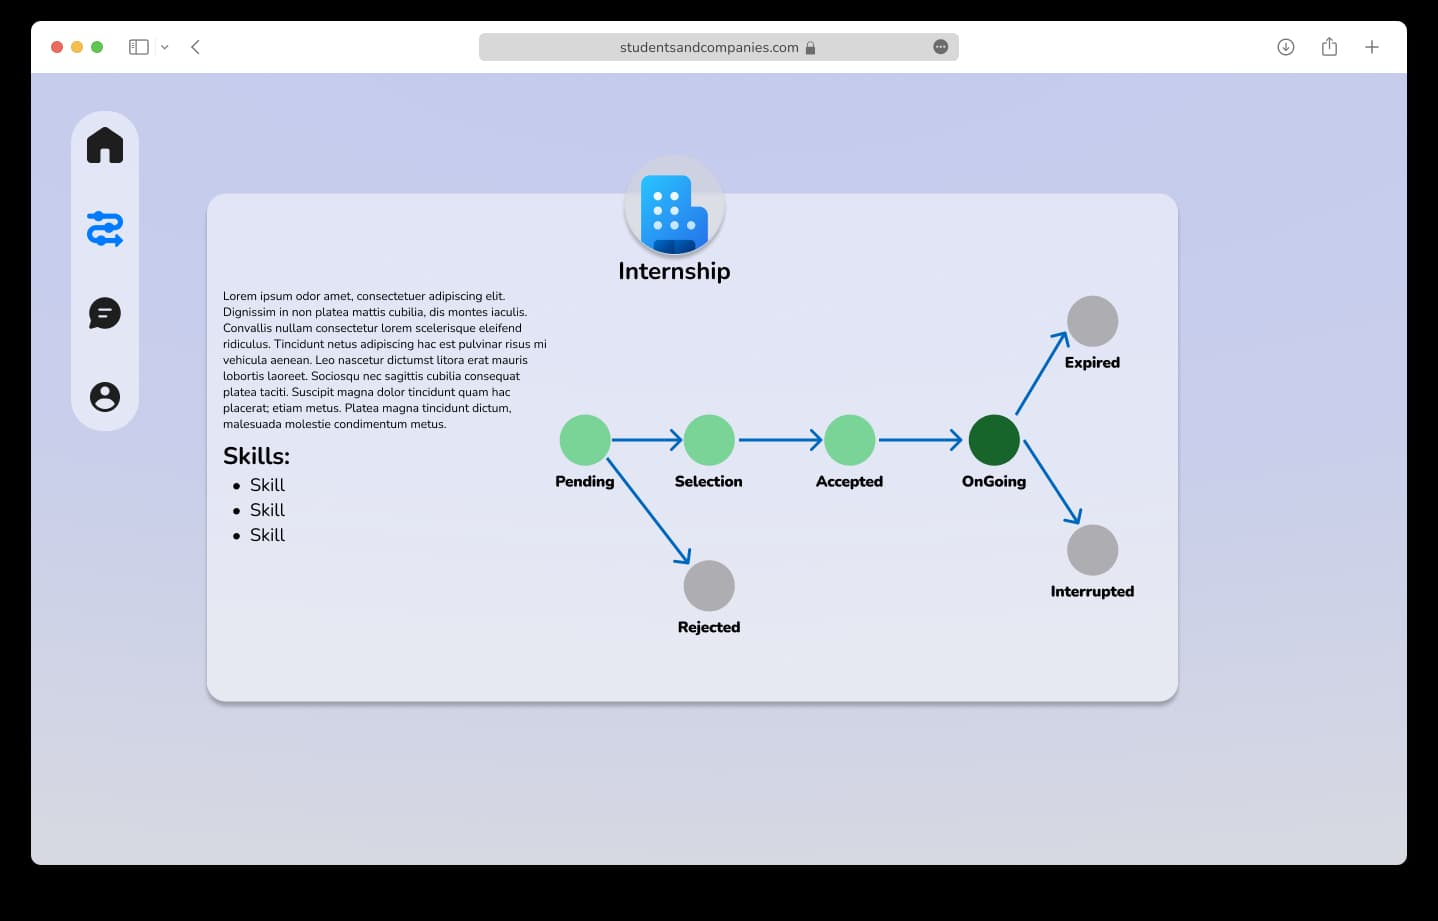
\includegraphics[width=\textwidth]{Images/MockUps/monitor_status.jpeg}
    \label{fig:enter-label}
\end{figure}
\subsubsection{Hardware Interfaces}
No hardware interfaces are provided, being S\&C just a software system.
\subsubsection{Software Interfaces}
In order to work the system needs some software interfaces.
\begin{itemize}
    \item \textbf{SheerID API}: in order to verify the students identity and his university, used also for user login.
\end{itemize}
\subsubsection{Communication Interfaces}
The system, which is entirely web-based, relies on HTTPS protocol.
\subsection{Functional Requirements}
\subsubsection{Student}
\paragraph{Login}
\begin{requirements}
\item The system must allow students to log-in through their academic email and password, if they provide them correctly.
\item Only students with an academic credential provided by a registered university can log-in.
\end{requirements}
\paragraph{Edit profile}
\begin{requirements}[resume]
\item The system must allow the student to edit his profile info, remove the CV and add a new version of the CV.
\item The student can edit only his profile.
\end{requirements}
\paragraph{Internship recommendation}
\begin{requirements}[resume]
\item The system must send an email to the student when an internship that might interest him becomes available.
\end{requirements}
\paragraph{Search an internship}
\begin{requirements}[resume]
\item The system must provide to the student all internships satisfying search criteria.
\item The system must provide to the student only internships satisfying search criteria.
\end{requirements}
\paragraph{Apply for an internship}
\begin{requirements}[resume]
\item The system must register the student's application for the internship.
\item The system must register only applications of students who have submitted an application for the internship.
\end{requirements}
\paragraph{Answer interview questions}
\begin{requirements}[resume]
\item The student must be able to answer interview questionnaires.
\item The student can answer interview questionnaires regarding only internships he’s applied for and accepted by the involved company.
\end{requirements}
\paragraph{Consulting CV suggestion}
\begin{requirements}[resume]
\item The student must be able to view suggestions on how to improve his CV.
\item The student can view suggestions regarding only his CV.
\end{requirements}
\subsubsection{Company}
\paragraph{Registration and login}
\begin{requirements}[resume]
\item The system must allow companies to register to S\&C providing mandatory data (name, email, VAT number) and selecting a password.
\item The system must allow registered companies to log-in through their email and password, if they are provided correctly. 
\end{requirements}
\paragraph{Upload an internship}
\begin{requirements}[resume]
\item The system must allow the company to fill an internship creation form.
\item The system must allow the company to select the internship type.
\item The system must allow the company to select the internship duration.
\item The system must allow the company to select if the internship is paid or not.
\item The system must allow the company to select the skills it is searching for in the candidates.
\end{requirements}
\paragraph{Student recommendation}
\begin{requirements}[resume]
\item The system must send an email notifying the company when a student with a CV corresponding to their needs becomes available.
\end{requirements}
\paragraph{Interview students}
\begin{requirements}[resume]
\item The company must be able to provide structured questionnaires to students.
\item The company can provide structured questionnaires only to students who have applied to an internship uploaded by the company itself.
\item The company must be able to view answers to questionnaires it created.
\end{requirements}
\paragraph{Create contract}
\begin{requirements}[resume]
\item The company must be able to register a contract regarding an internship and referring to the assigned student.
\item The company can register contracts regarding only internships uploaded by the company itself.
\item The company can register contracts referring only to students that have applied for the indicated internship.
\end{requirements}
\subsubsection{University}
\paragraph{Login}
\begin{requirements}[resume]
\item The system must allow registered universities to log-in through credentials provided by S\&C, if they are provided correctly.
\end{requirements}
\paragraph{Terminate an internship}
\begin{requirements}[resume]
\item The system must allow universities to terminate an internship involving their students.
\end{requirements}
\subsubsection{Students and Companies}
\paragraph{Leave a feedback}
\begin{requirements}[resume]
\item The student must be able to post a feedback.
\item The company must be able to post a feedback.
\item Only students that have participated in an internship can leave feedback for it.
\item Only companies that have participated in an internship can leave feedback for it.
\item Every student can leave at most one feedback per internship.
\item Every company can leave at most one feedback per internship.
\end{requirements}
\paragraph{Open discussion}
\begin{requirements}[resume]
\item The student must be able to open a discussion with the company he’s interning with and the university he’s enrolled at.
\item The company must be able to open a discussion with the students they are collaborating with and universities those students are enrolled at.
\item The student can open a discussion only with the company he’s interning with and the university he’s enrolled at.
\item The company can open a discussion only with students they are collaborating with and  universities.
\end{requirements}
\subsubsection{Everyone}
\begin{requirements}[resume]
\item The student can send and receive messages only from a discussion he is participating in.
\item The company can send and receive messages only from a discussion it is participating in.
\item The university can send and receive messages only from a discussion it is participating in.
\item The student must be able to monitor the status of the internships in which he has applied.
\item The company must be able to monitor the status of the internships it has published.
\item The university must be able to monitor the status of the internship in which its students have applied.
\end{requirements}




\subsubsection{Use Cases Diagram}
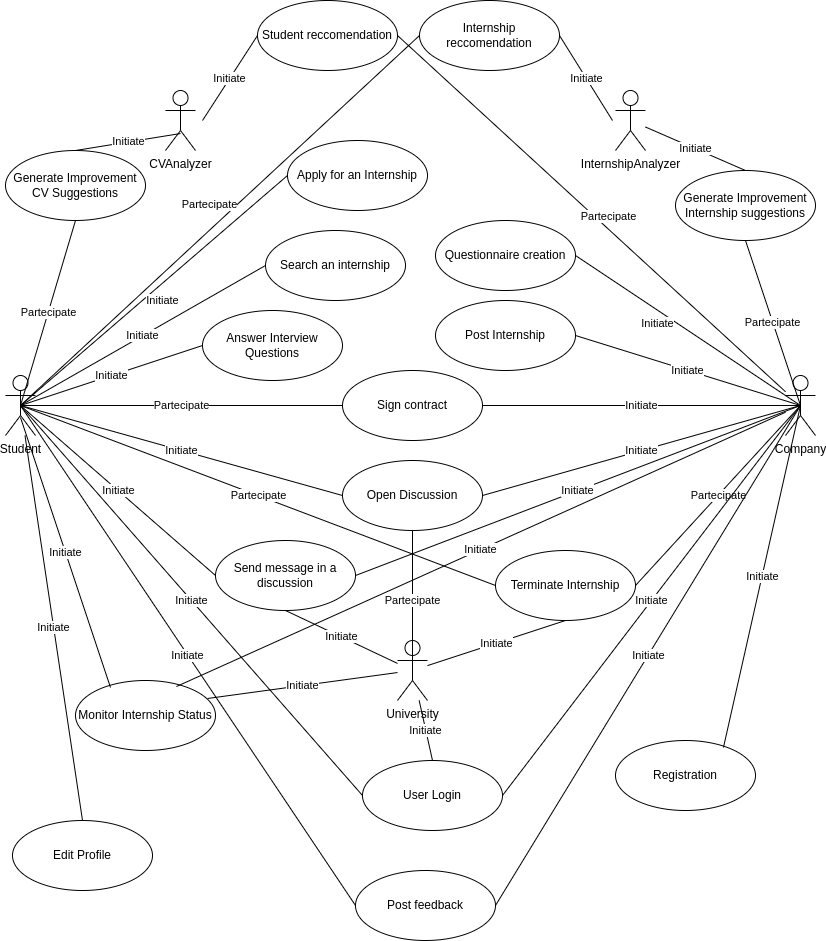
\includegraphics[width=\textwidth]{Images/use_cases.png}
\subsubsection{Use Cases}
\begin{use-case}
    \item Company Registration\\
        \uctab{Company registration}{
                \begin{itemize}
                    \item Company
                \end{itemize}
            }{The company has clicked the register button in the login view.}{
              \begin{enumerate}
                  \item The user presses the register button.
                  \item The system shows the registration form.
                  \item The user compiles the form.
                  \item The user presses the submit button.
                  \item The platform shows the dashboard.
              \end{enumerate}  
            }{The company has successfully registered to the platform.}{
                \begin{itemize}
                    \item There are missing data.
                    \item There already exists a user with those credentials.
                    \item Data format is not valid.
                \end{itemize}
            }
    \item Company Login\\
        \uctab{Company Login}{
                \begin{itemize}
                    \item Company
                \end{itemize}
            }{The company has opened the S\&C platform.}{
              \begin{enumerate}
                  \item The company fills the form.
                  \item The company clicks the submit button.
                  \item The platform shows the dashboard.
              \end{enumerate}  
            }{The company has successfully logged into the platform}{There does not exist any company with the submitted credentials.}
    \item University Login\\
        \uctab{University Login}{
                \begin{itemize}
                    \item University
                \end{itemize}
            }{The university has opened the S\&C platform.}{
              \begin{enumerate}
                  \item The university fills the form.
                  \item The university clicks the submit button.
                  \item The platform shows the dashboard.
              \end{enumerate}  
            }{The university has successfully logged into the platform.}{
                There does not exist any university with the submitted credentials.
            }
    \item Student Login\\
    \uctab{Student Login}{
                \begin{itemize}
                    \item Student
                    \item SheerID
                \end{itemize}
            }{The student has opened the S\&C platform.}{
              \begin{enumerate}
                  \item The student fills the form.
                  \item The student clicks the submit button.
                  \item The platform shows the dashboard.
              \end{enumerate}  
            }{The student has successfully logged into the platform.}{
                There does not exist any student with the submitted credentials.
            }
    \item Post Internship\\
    \uctab{Post Internship}{
                \begin{itemize}
                    \item Company
                \end{itemize}
            }{The company is logged to the S\&C platform.}{
              \begin{enumerate}
                  \item The company clicks the upload internship button.
                  \item The company fills the form with the information about the internship: title, description, requested skills and the interview questionnaire.
              \end{enumerate}  
            }{The internship is successfully uploaded on the platform.}{}
    \item Post Feedback\\
    \uctab{Post Feedback}{
                \begin{itemize}
                    \item Student
                    \item Company
                \end{itemize}
            }{The user is logged in and on the page of an internship he was involved in.}{
              \begin{enumerate}
                  \item The user clicks on the post feedback button.
                  \item The user fills the form with a rating and, optionally, a comment.
                  \item The user clicks on the submit button.
              \end{enumerate}  
            }{The feedback is successfully uploaded on the platform.}{
                A required field was not filled.
            }
    \item Search an Internship\\
    \uctab{Search an Internship}{
                \begin{itemize}
                    \item Student
                \end{itemize}
            }{The student is logged to the S\&C platform.}{
              \begin{enumerate}
                  \item The student clicks the search icon.
                  \item The student selects any search criteria or filters.
                  \item The system displays the internships of the student that meet the selected filters, if any.
              \end{enumerate}  
            }{Internships are displayed to the student.}{}
    \item Apply for an Internship\\
    \uctab{Apply for an Internship}{
                \begin{itemize}
                    \item Student
                \end{itemize}
            }{The student is logged to the S\&C platform.}{
              \begin{enumerate}
                  \item The student clicks on an internship post.
                  \item The student clicks the "apply for the internship" button.
              \end{enumerate}  
            }{The student has applied successfully for the internship.}{}
    \item Questionnaire Creation\\
    \uctab{Questionnaire Creations}{
                \begin{itemize}
                    \item Company
                \end{itemize}
            }{The company is logged to the S\&C platform.}{
              \begin{enumerate}
                  \item The company clicks the create questionnaire button.
                  \item The company fills the form with the questions to be inserted into the questionnaire.
                  \item The company clicks the submit button.
              \end{enumerate}  
            }{The questionnaire is successfully sent to the all the applicants.}{}
    \item Answer Questionnaire Interview\\
    \uctab{Answer Questionnaire Interview}{
                \begin{itemize}
                    \item Student
                \end{itemize}
            }{The student is logged to the S\&C platform and there exists a contract between both parties.}{
              \begin{enumerate}
                  \item The student clicks on the answer questions button.
                  \item The system shows the questions to the student,
                  \item The student answer the questions.
                  \item The student clicks the submit button.
              \end{enumerate}  
            }{The questionnaire is successfully submitted and sent to the company.}{}
    \item Sign Contract\\
    \uctab{Sign Contract}{
                \begin{itemize}
                    \item Company
                \end{itemize}
            }{The company is logged to the S\&C platform and has received the applicant's questionnaire answers.}{
              \begin{enumerate}
                  \item The company selects the internship and the applicant to begin working with.
                  \item The company clicks the create contract button.
                  \item The company uploads the contract.
              \end{enumerate}  
            }{The student can start his internship.}{Invalid contract format.}
    \item Open Discussion\\
    \uctab{Open Discussion}{
                \begin{itemize}
                    \item Student
                    \item Company
                \end{itemize}
            }{The user is logged to the S\&C platform and there exists a contract between both parties.}{
              \begin{enumerate}
                  \item The user clicks on the open discussion button.
                  \item The user insert a title for the discussion.
                  \item The user clicks the submit button.
              \end{enumerate}  
            }{The discussion is successfully created.}{}
    \item Send Message in a Discussion\\
    \uctab{Send Message in a Discussion}{
                \begin{itemize}
                    \item User
                \end{itemize}
            }{The user must be logged to the S\&C platform and be involved in an internship discussion.}{
              \begin{enumerate}
                  \item The user clicks on the internship.
                  \item The user clicks on the discussion.
                  \item The user writes a message.
                  \item The user clicks the send button.
                  \item The system sends the updated discussion view.
              \end{enumerate}  
            }{The message is sent and all the involved users can now see it, if logged in, in the discussion section.}{}
    \item Terminate Internship\\
    \uctab{Terminate Internship}{
                \begin{itemize}
                    \item Student
                    \item Company
                    \item University
                \end{itemize}
            }{The university is logged to the S\&C platform and there exists an internship contract between the student and the company.}{
              \begin{enumerate}
                  \item The university clicks on the internship.
                  \item The university clicks the "terminate internship" button.
                  \item A notification is sent to the involved student.
                  \item A notification is sent to the involved company.
                  \item A notification is sent to the university.
              \end{enumerate}  
            }{The internship is now terminated.}{}
    \item Generate Improvement CV Suggestion\\
    \uctab{Generate Improvement CV Suggestion}{
                \begin{itemize}
                    \item Student.
                \end{itemize}
            }{A CV/internship has been added/updated.}{
              \begin{enumerate}
                  \item The system analyzes existing CVs and internships.
                  \item The system generates, if possible, a suggestion.
                  \item The system sends to the students an email with suggestions on how to improve the CV.
              \end{enumerate}  
            }{The student has received a suggestion on how to improve his CV.}{}
    \item Generate Internship Improvement Suggestion\\
    \uctab{Generate Improvement Internship Suggestions}{
                \begin{itemize}
                    \item Company.
                \end{itemize}
            }{A CV/internship has been added/updated.}{
              \begin{enumerate}
                  \item The system analyzes existing CVs and internships.
                  \item The system generates, if possible, a suggestion.
                  \item The system sends to the company an email with suggestions on how to improve the internship.
              \end{enumerate}  
            }{The company has received a suggestion on how to improve their internship.}{}
    \item Student Recommendation\\
    \uctab{Student Recommendation}{
                \begin{itemize}
                    \item Company
                \end{itemize}
            }{A CV has been added/updated.}{
              \begin{enumerate}
                  \item The system analyzes the CV.
                  \item If the system finds out that the CV might be interesting to a company, it sends an email to the company notifying the availability,
              \end{enumerate}  
            }{The company has received a notification about the availability of a new CV.}{}
    \item Internship Recommendation\\
    \uctab{Internship Recommendation}{
                \begin{itemize}
                    \item Student
                \end{itemize}
            }{An internship has been added.}{
              \begin{enumerate}
                  \item The system analyzes the new internship.
                  \item If the system finds that the new internship might interest a student, it sends an email to that student notifying the availability.
              \end{enumerate}  
            }{The company has received a notification about the availability of a new CV.}{}
    \item Monitor Internship Status\\
    \uctab{Monitor Internship Status}{
                \begin{itemize}
                    \item User
                \end{itemize}
            }{The user is either a student, a company or a university involved directly in an active internship.}{
              \begin{enumerate}
                  \item The user clicks on the internship to monitor.
                  \item The system shows the internship status and the eventual discussions.
              \end{enumerate}  
            }{The system has shown the internship dashboard with info.}{}
    \item Edit Profile\\
    \uctab{Edit Profile}{
                \begin{itemize}
                    \item Student
                \end{itemize}
            }{The student is logged to the S\&C platform.}{
              \begin{enumerate}
                  \item The student clicks on the "edit profile" button.
                  \item The student selects the fields to modify, this includes the possibility to select the CV field.
                  \item The student changes the data in the selected fields. If the CV field was selected, the student uploads the new version of the CV.
                  \item The student clicks on the save button.
              \end{enumerate}  
            }{The system registers the new data}{The student clicks the "cancel" button. Old data recorded in the system is preserved.}
\end{use-case}
\subsubsection{Sequence Diagrams}
\begin{use-case}
    \item Company Registration\\
    
\includegraphics[width=0.5\textwidth]{Images/Use Cases/company_registration.png}\\
    \item Company Login\\
    
\includegraphics[width=0.5\textwidth]{Images/Use Cases/company_login.png}\\
    \item University Login\\
    
\includegraphics[width=0.5\textwidth]{Images/Use Cases/university_login.png}\\
    \item Student Login\\
    
\includegraphics[width=0.5\textwidth]{Images/Use Cases/student_login.png}\\
    \item Post Internship\\
    
\includegraphics[width=0.5\textwidth]{Images/Use Cases/post_internship.png}\\
    \item Post Feedback\\
    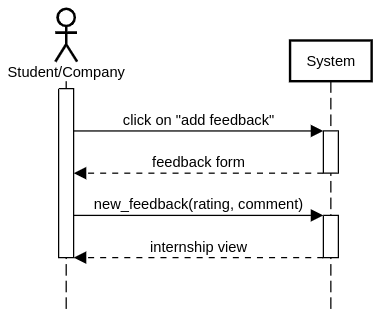
\includegraphics[width=0.5\textwidth]{Images/Use Cases/giving_feedback.png}\\
    \item Search an Internship\\
    
\includegraphics[width=0.5\textwidth]{Images/Use Cases/search_internship.png}\\
    \item Apply for an Internship\\
    
\includegraphics[width=0.5\textwidth]{Images/Use Cases/apply_internship.png}\\
    \item Questionnaire Creation\\
    
\includegraphics[width=0.5\textwidth]{Images/Use Cases/questionnaire_creation.png}\\
    \item Answer Questionnaire Interview\\
    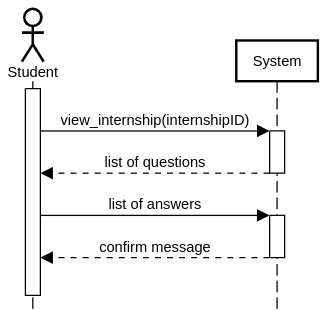
\includegraphics[width=0.5\textwidth]{Images/Use Cases/questionnaire_submit.png}\\
    \item Sign Contract\\
    
\includegraphics[width=0.5\textwidth]{Images/Use Cases/sign_contract.png}\\
    \item Open Discussion\\
    
\includegraphics[width=0.5\textwidth]{Images/Use Cases/open_discussion.png}\\
    \item Send Message in a Discussion\\
    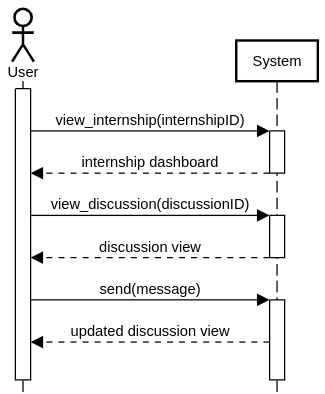
\includegraphics[width=0.5\textwidth]{Images/Use Cases/discussion_message.png}\\
    \item Terminate Internship\\
    
\includegraphics[width=0.5\textwidth]{Images/Use Cases/terminate_internship.png}\\
    \item Generate CV Improvement Suggestion\\
    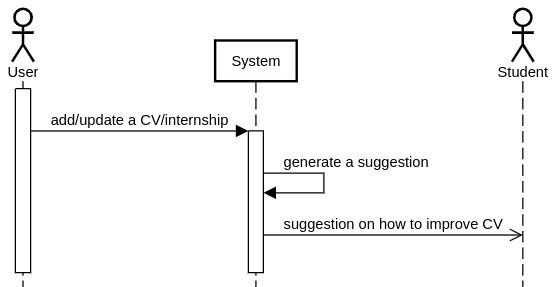
\includegraphics[width=0.5\textwidth]{Images/Use Cases/CV_suggestion.png}\\
    \item Generate Internship Improvement Suggestion\\
    
\includegraphics[width=0.5\textwidth]{Images/Use Cases/internship_suggestion.png}\\
    \item Student Recommendation\\
    
\includegraphics[width=0.5\textwidth]{Images/Use Cases/student_recommendation.png}\\
    \item Internship Recommendation\\
    
\includegraphics[width=0.5\textwidth]{Images/Use Cases/internship_recommendation.png}\\
    \item Monitor Internship Status\\
    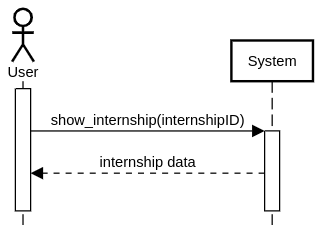
\includegraphics[width=0.5\textwidth]{Images/Use Cases/monitor_internship_status.png}\\
    \item Edit Profile\\
    
\includegraphics[width=0.5\textwidth]{Images/Use Cases/edit_profile.png}\\
\end{use-case}
\subsubsection{Requirement Mapping}
\reqmap{
\multicolumn{2}{|p{\textwidth}|}{{[G1]} Students must be able to search for internships posted by companies} \\
\hline
{[R]} The system must allow companies to register to S\&C providing mandatory data (name, email, P.IVA) and selecting a password. & {[D1]} Students create their CVs \\
{[R]} The system must allow registered companies to log-in through their email and password, if they are provided correctly.  & {[D2]} Companies properly insert informations about internships \\
{[R]} The system must allow the company to fill an internship creation form. & {[D6]} Students have an academic credential. \\
{[R]} The system must allow the company to select the internship type. & {[D7]} University is available on the SheerID API. \\
{[R]} The system must allow the company to select the internship duration. & {[D8]} Students are enrolled in a university registered on SheerID. \\
{[R]} The system must allow the company to select if the internship is paid or not. & {[D9]} Users who register as a company have a valid VAT number. \\
{[R]} The system must allow the company to select the skills it is searching for in the candidates. & ~ \\
{[R]} The system must allow students to log-in through their academic email and password, if they provide them correctly. & ~ \\
{[R]} Only students with an academic credential provided by a registered university can log-in. & ~ \\
{[R]} The system must provide to the student all internships satisfying search criteria. & ~ \\
{[R]} The system must provide to the student only internships satisfying search criteria. & ~ \\
}
\\ \\ \\
\reqmap{
\multicolumn{2}{|p{\textwidth}|}{{[G2]} Companies must be able to upload their internships offers} \\
\hline
{[R]} The system must allow companies to register to S\&C providing mandatory data (name, email, P.IVA) and selecting a password. & {[D2]} Companies properly insert information about internships. \\
{[R]} The system must allow registered companies to log-in through their email and password, if they are provided correctly.  & {[D9]} Users who register as a company have a valid VAT number. \\
{[R]} The system must allow the company to fill an internship creation form. & ~ \\
{[R]} The system must allow the company to select the internship type. & ~ \\
{[R]} The system must allow the company to select the internship duration. & ~ \\
{[R]} The system must allow the company to select if the internship is paid or not. & ~ \\
{[R]} The system must allow the company to select the skills it is searching for in the candidates. & ~ \\
}
\\ \\ \\
\reqmap{
\multicolumn{2}{|p{\textwidth}|}{{[G3]} Students must be notified when an internship that could interest them becomes available.} \\
\hline
{[R]} The system must allow students to log-in through their academic email and password, if they provide them correctly. & {[D2]} Companies properly insert information about internships. \\
{[R]} Only students with an academic credential provided by a registered university can log-in. & {[D4]} Notifications must arrive to the target users. \\
{[R]} The system must provide to the student all internships satisfying search criteria. & {[D6]} Students have an academic credential. \\
{[R]} The system must provide to the student only internships satisfying search criteria. & {[D7]} University is available on the SheerID API. \\
~ & {[D8]} Students are enrolled in a university registered on SheerID. \\
}
\\ \\ \\
\reqmap{
\multicolumn{2}{|p{\textwidth}|}{{[G4]} Companies must be notified about available students with CVs and skills matching their internship requirements.} \\
\hline
{[R]} The system must allow companies to register to S\&C providing mandatory data (name, email, P.IVA) and selecting a password. & {[D1]} Students create their CVs. \\
{[R]} The system must allow registered companies to log-in through their email and password, if they are provided correctly.  & {[D2]} Companies properly insert information about internships. \\
{[R]} The system must allow the company to fill an internship creation form. & {[D4]} Notifications must arrive to the target users. \\
{[R]} The system must allow the company to select the internship type. & {[D9]} Users who register as a company have a valid VAT number. \\
{[R]} The system must allow the company to select the internship duration. & ~ \\
{[R]} The system must allow the company to select if the internship is paid or not. & ~ \\
{[R]} The system must allow the company to select the skills it is searching for in the candidates. & ~ \\
{[R]} The system must send an email notifying the company when a student with a CV corresponding to their needs becomes available. & ~ \\
}
\\ \\ \\
\reqmap{
\multicolumn{2}{|p{\textwidth}|}{{[G5]} Students must be able to apply for internships of interest.} \\
\hline
{[R]} The system must allow students to log-in through their academic email and password, if they provide them correctly. & {[D1]} Students create their CVs. \\
{[R]} Only students with an academic credential provided by a registered university can log-in. & {[D2]} Companies properly insert information about internships. \\
{[R]} The system must provide to the student all internships satisfying search criteria. & {[D6]} Students have an academic credential. \\
{[R]} The system must provide to the student only internships satisfying search criteria. & {[D7]} University is available on the SheerID API. \\
~ & {[D8]} Students are enrolled in a university registered on SheerID. \\
}
\\ \\ \\
\reqmap{
\multicolumn{2}{|p{\textwidth}|}{{[G6]} Companies must be able to accept applicants to their internship.} \\
\hline
{[R]} The system must allow companies to register to S\&C providing mandatory data (name, email, P.IVA) and selecting a password. & {[D2]} Companies properly insert information about internships. \\
{[R]} The system must allow registered companies to log-in through their email and password, if they are provided correctly.  & ~ \\
{[R]} The company must be able to register a contract regarding an internship and referring to the assigned student. & ~ \\
{[R]} The company can register contracts regarding only internships uploaded by the company itself. & ~ \\
{[R]} The company can register contracts referring only to students that have applied for the indicated internship. & ~ \\
}
\\ \\ \\
\reqmap{
\multicolumn{2}{|p{\textwidth}|}{{[G7]} Companies must be supported in conducting a selection process for applicants, including the collection of information about the students using questionnaires and the management of interviews.} \\
\hline
{[R]} The system must allow students to log-in through their academic email and password, if they provide them correctly. & {[D1]} Students create their CVs. \\
{[R]} Only students with an academic credential provided by a registered university can log-in. & {[D2]} Companies properly insert information about internships. \\
{[R]} The student must be able to answer interview questionnaires. & {[D4]} Notifications must arrive to the target users. \\
{[R]} The student can answer interview questionnaires regarding only internships he’s applied for and accepted by the involved company. & {[D6]} Students have an academic credential. \\
{[R]} The system must allow companies to register to S\&C providing mandatory data (name, email, P.IVA) and selecting a password. & {[D7]} University is available on the SheerID API. \\
{[R]} The system must allow registered companies to log-in through their email and password, if they are provided correctly.  & {[D8]} Students are enrolled in a university registered on SheerID. \\
{[R]} The system must allow the company to fill an internship creation form. & {[D9]} Users who register as a company have a valid VAT number. \\
{[R]} The system must allow the company to select the internship type. & ~ \\
{[R]} The system must allow the company to select the internship duration. & ~ \\
{[R]} The system must allow the company to select if the internship is paid or not. & ~ \\
{[R]} The system must allow the company to select the skills it is searching for in the candidates. & ~ \\
{[R]} The company must be able to provide structured questionnaires to students. & ~ \\
{[R]} The company can provide structured questionnaires only to students who’ve applied to an internship uploaded by the company itself. & ~ \\
{[R]} The company must be able to view answers to questionnaires it created. & ~ \\
}
\\ \\ \\
\reqmap{
\multicolumn{2}{|p{\textwidth}|}{{[G8]} Students want to receive suggestions on how to make their CVs more appealing.} \\
\hline
{[R]} The system must allow students to log-in through their academic email and password, if they provide them correctly. & {[D1]} Students create their CVs. \\
{[R]} Only students with an academic credential provided by a registered university can log-in. & {[D2]} Companies properly insert information about internships. \\
{[R]} The system must provide to the student all internships satisfying search criteria. & {[D4]} Notifications must arrive to the target users. \\
{[R]} The system must provide to the student only internships satisfying search criteria. & {[D6]} Students have an academic credential. \\
{[R]} The student must be able to view suggestions on how to improve his CV. & {[D7]} University is available on the SheerID API. \\
{[R]} The student can view suggestions regarding only his CV. & {[D8]} Students are enrolled in a university registered on SheerID. \\
{[R]} The system must allow companies to register to S\&C providing mandatory data (name, email, P.IVA) and selecting a password. & {[D9]} Users who register as a company have a valid VAT number. \\
{[R]} The system must allow registered companies to log-in through their email and password, if they are provided correctly.  & ~ \\
{[R]} The system must allow the company to fill an internship creation form. & ~ \\
{[R]} The system must allow the company to select the internship type. & ~ \\
{[R]} The system must allow the company to select the internship duration. & ~ \\
{[R]} The system must allow the company to select if the internship is paid or not. & ~ \\
{[R]} The system must allow the company to select the skills it is searching for in the candidates. & ~ \\
}
\\ \\ \\
\reqmap{
\multicolumn{2}{|p{\textwidth}|}{{[G9]} Companies want to receive suggestions on how to make their project descriptions more appealing.} \\
\hline
{[R]} The system must allow companies to register to S\&C providing mandatory data (name, email, P.IVA) and selecting a password. & {[D2]} Companies properly insert information about internships. \\
{[R]} The system must allow registered companies to log-in through their email and password, if they are provided correctly.  & {[D4]} Notifications must arrive to the target users. \\
{[R]} The system must allow the company to fill an internship creation form. & {[D9]} Users who register as a company have a valid VAT number. \\
{[R]} The system must allow the company to select the internship type. & ~ \\
{[R]} The system must allow the company to select the internship duration. & ~ \\
{[R]} The system must allow the company to select if the internship is paid or not. & ~ \\
{[R]} The system must allow the company to select the skills it is searching for in the candidates. & ~ \\
}
\\ \\ \\
\reqmap{
\multicolumn{2}{|p{\textwidth}|}{[G10.A] Students must be able to keep track and monitor the execution and the outcomes of the matchmaking process.} \\
\hline
{[R]} The system must allow students to log-in through their academic email and password, if they provide them correctly. & {[D1]} Students create their CVs. \\
{[R]} Only students with an academic credential provided by a registered university can log-in. & {[D2]} Companies properly insert information about internships. \\
{[R]} The system must provide to the student all internships satisfying search criteria. & {[D4]} Notifications must arrive to the target users. \\
{[R]} The system must provide to the student only internships satisfying search criteria. & {[D6]} Students have an academic credential. \\
{[R]} The system must register the student's application for the internship. & {[D7]} University is available on the SheerID API. \\
{[R]} The system must register only applications of students who have submitted an application for the internship. & {[D8]} Students are enrolled in a university registered on SheerID. \\
{[R]} The student must be able to monitor the status of the internships in which he has applied. & {[D9]} Users who register as a company have a valid VAT number. \\
{[R]} The company must be able to monitor the status of the internships it has published. & ~ \\
{[R]} The university must be able to monitor the status of the internship in which its students have applied. & ~ \\
}
\\ \\ \\
\reqmap{
\multicolumn{2}{|p{\textwidth}|}{[G10.B] Companies must be able to keep track and monitor the execution and the outcomes of the matchmaking process.} \\
\hline
{[R]} The system must allow companies to register to S\&C providing mandatory data (name, email, P.IVA) and selecting a password. & {[D1]} Students create their CVs. \\
{[R]} The system must allow registered companies to log-in through their email and password, if they are provided correctly.  & {[D2]} Companies properly insert information about internships. \\
{[R]} The system must allow the company to fill an internship creation form. & {[D4]} Notifications must arrive to the target users. \\
{[R]} The system must allow the company to select the internship type. & {[D6]} Students have an academic credential. \\
{[R]} The system must allow the company to select the internship duration. & {[D7]} University is available on the SheerID API. \\
{[R]} The system must allow the company to select if the internship is paid or not. & {[D8]} Students are enrolled in a university registered on SheerID. \\
{[R]} The system must allow the company to select the skills it is searching for in the candidates. & {[D9]} Users who register as a company have a valid VAT number. \\
{[R]} The system must send an email notifying the company when a student with a CV corresponding to their needs becomes available. & ~ \\
{[R]} The student must be able to monitor the status of the internships in which he has applied. & ~ \\
{[R]} The company must be able to monitor the status of the internships it has published. & ~ \\
{[R]} The university must be able to monitor the status of the internship in which its students have applied. & ~ \\
}
\\ \\ \\
\reqmap{
\multicolumn{2}{|p{\textwidth}|}{[G10.C] Universities must be able to monitor the status of the internship in which its students have applied.} \\
\hline
{[R]} The system must register the student's application for the internship. & {[D1]} Students create their CVs. \\
{[R]} The system must register only applications of students who have submitted an application for the internship. & {[D2]} Companies properly insert information about internships. \\
{[R]} The system must allow the company to fill an internship creation form. & {[D3]} Universities interfere with the contract between students and companies when needed. \\
{[R]} The system must allow the company to select the internship type. & {[D4]} Notifications must arrive to the target users. \\
{[R]} The system must allow the company to select the internship duration. & {[D6]} Students have an academic credential. \\
{[R]} The system must allow the company to select if the internship is paid or not. & {[D7]} University is available on the SheerID API. \\
{[R]} The system must allow the company to select the skills it is searching for in the candidates. & {[D8]} Students are enrolled in a university registered on SheerID. \\
{[R]} The system must allow registered universities to log-in through credentials provided by S\&C, if they are provided correctly.  & {[D9]} Users who register as a company have a valid VAT number. \\
{[R]} The student must be able to monitor the status of the internships in which he has applied. & ~ \\
{[R]} The company must be able to monitor the status of the internships it has published. & ~ \\
{[R]} The university must be able to monitor the status of the internship in which its students have applied. & ~ \\
}
\\ \\ \\
\reqmap{
\multicolumn{2}{|p{\textwidth}|}{{[G11]} The interested parties of an internship (students, companies and universities) must be able to communicate with each other about info and eventual problems regarding the ongoing internship.} \\
\hline
{[R]} The system must allow students to log-in through their academic email and password, if they provide them correctly. & {[D3]} Universities interfere with the contract between students and companies when needed. \\
{[R]} Only students with an academic credential provided by a registered university can log-in. & {[D4]} Notifications must arrive to the target users. \\
{[R]} The system must allow companies to register to S\&C providing mandatory data (name, email, P.IVA) and selecting a password. & {[D6]} Students have an academic credential. \\
{[R]} The system must allow registered companies to log-in through their email and password, if they are provided correctly.  & {[D7]} University is available on the SheerID API. \\
{[R]} The system must allow registered universities to log-in through credentials provided by S\&C, if they are provided correctly. & {[D8]} Students are enrolled in a university registered on SheerID. \\
{[R]} The student must be able to open a discussion with the company he’s interning with and the university he’s enrolled at. & ~ \\
{[R]} The company must be able to open a discussion with the students they are collaborating with and universities those students are enrolled at. & ~ \\
{[R]} The student can open a discussion only with the company he’s interning with and the university he’s enrolled at. & ~ \\
{[R]} The company can open a discussion only with students they are collaborating with and  universities. & ~ \\
{[R]} The student can send and receive messages only from a discussion he is participating in. & ~ \\
{[R]} The company can send and receive messages only from a discussion it is participating in. & ~ \\
{[R]} The university can send and receive messages only from a discussion it is participating in. & ~ \\
}
\\ \\ \\
\reqmap{
\multicolumn{2}{|p{\textwidth}|}{[G12.A] Companies must be able to file complaints about students interning with them.} \\
\hline
{[R]} The system must allow companies to register to S\&C providing mandatory data (name, email, P.IVA) and selecting a password. & {[D3]} Universities interfere with the contract between students and companies when needed. \\
{[R]} The system must allow registered companies to log-in through their email and password, if they are provided correctly.  & {[D4]} Notifications must arrive to the target users. \\
{[R]} The company must be able to open a discussion with the students they are collaborating with and universities those students are enrolled at. & {[D9]} Users who register as a company have a valid VAT number. \\
{[R]} The company can open a discussion only with students they are collaborating with and  universities. & ~ \\
{[R]} The student can send and receive messages only from a discussion he is participating in. & ~ \\
{[R]} The company can send and receive messages only from a discussion it is participating in. & ~ \\
{[R]} The university can send and receive messages only from a discussion it is participating in. & ~ \\
}
\\ \\ \\
\reqmap{
\multicolumn{2}{|p{\textwidth}|}{[G12.B] Students must be able to file complaints about the companies where they are interning.} \\
\hline
{[R]} The system must allow students to log-in through their academic email and password, if they provide them correctly. & {[D3]} Universities interfere with the contract between students and companies when needed. \\
{[R]} Only students with an academic credential provided by a registered university can log-in. & {[D4]} Notifications must arrive to the target users. \\
{[R]} The student must be able to open a discussion with the company he’s interning with and the university he’s enrolled at. & {[D6]} Students have an academic credential. \\
{[R]} The student can open a discussion only with the company he’s interning with and the university he’s enrolled at. & {[D7]} University is available on the SheerID API. \\
{[R]} The student can send and receive messages only from a discussion he is participating in. & {[D8]} Students are enrolled in a university registered on SheerID. \\
{[R]} The company can send and receive messages only from a discussion it is participating in. & ~ \\
{[R]} The university can send and receive messages only from a discussion it is participating in. & ~ \\
}
\\ \\ \\
\reqmap{
\multicolumn{2}{|p{\textwidth}|}{{[G13]} Universities must be able to review complaints about their students and the companies where their students are interning.} \\
\hline
{[R]} The system must allow registered universities to log-in through credentials provided by S\&C, if they are provided correctly. & {[D3]} Universities interfere with the contract between students and companies when needed. \\
{[R]} The company must be able to open a discussion with the students they are collaborating with and universities those students are enrolled at. & {[D4]} Notifications must arrive to the target users. \\
{[R]} The company can open a discussion only with students they are collaborating with and  universities. & {[D6]} Students have an academic credential. \\
{[R]} The company can only send and receive messages from a discussion it is participating in. & {[D7]} University is available on the SheerID API. \\
{[R]} The university can only send and receive messages from a discussion it is participating in. & {[D8]} Students are enrolled in a university registered on SheerID. \\
}
\\ \\ \\
\reqmap{
\multicolumn{2}{|p{\textwidth}|}{{[G14]} Universities must be able to interrupt internships between their students and a company.} \\
\hline
{[R]} The system must allow registered universities to log-in through credentials provided by S\&C, if they are provided correctly. & {[D3]} Universities interfere with the contract between students and companies when needed. \\
{[R]} The system must allow universities to terminate an internship involving their students & {[D4]} Notifications must arrive to the target users. \\
{[R]} The student must be able to open a discussion with the company he’s interning with and the university he’s enrolled at. & {[D6]} Students have an academic credential. \\
{[R]} The company must be able to open a discussion with the students they are collaborating with and universities those students are enrolled at. & {[D7]} University is available on the SheerID API. \\
{[R]} The student can open a discussion only with the company he’s interning with and the university he’s enrolled at. & {[D8]} Students are enrolled in a university registered on SheerID. \\
{[R]} The company can open a discussion only with students they are collaborating with and  universities. & ~ \\
}
\subsection{Performance Requirements}
Performance requirements are not particularly critical for the system, but it is anyway desirable that all requests sent to the server are answered within 1 second, to assure a good user experience.\\
The server infrastructure will be designed to be scalable so that it will be possible to adapt it to the increment of users when the app diffusion will increase.
\subsection{Design Constraints}
\subsubsection{Standards Compliance}
The CKB platform pays a great attention for what concerns users privacy cause of this
the CKB project is in compliance with the General Data Protection Regulation (GPDR)
a regulation in EU law on data protection and privacy for all individuals within the
European Union (EU) and the European Economic Area (EEA). Moreover, the platform
has to use the international format of date and time to adequate to the newer standards.

\subsubsection{Hardware and Software Limitations}
There are not significant limitations since users can access the system using every modern browser
\subsection{Software System Attributes}
\subsubsection{Availability}
The availability is not a critical requirement, but the system has to guarantee a 99\% of uptime (max 3.65 days/year of downtime) to ensure that the users can normally use it.
\subsubsection{Security}
Security is a critical requirement for this system, considering the confidential information that is transmitted through it. It is assured by the use of the HTTPS protocol for all communications and by following the best security practices for the servers management, maintaining the data ciphered and assuring the access only to the authorized users.
\subsubsection{Maintainability}
The system will be realized following the best software engineering practices to ensure its maintainability and expandability in the future.
\subsubsection{Portability}
The system is a web application so it must be compatible with modern web browsers
(Firefox, Google Chrome and so on) and feature a responsive interface to be used on a wide range of screen formats (smartphones, tablets, computers, etc).